\documentclass{article}
\usepackage{float}  % Improves float positioning
\usepackage{multirow}  % Merges rows in tables
\usepackage{tabularx}  % Auto-adjust column widths
\usepackage{caption}  % Customizes captions
\usepackage{adjustbox}  % Adjusts box size/position
\usepackage{xltabular}  % Multi-page tables support
\usepackage{enumitem}  % Customizes lists
\usepackage{makecell}  % Multi-line table cells
\usepackage{animate}  % Enables animations
\usepackage{longtable}  % Tables across pages
\usepackage{graphicx}  % Includes graphics
\usepackage{multicol}  % Multi-column text
\usepackage{comment}  % Block comments
\usepackage[absolute,overlay]{textpos}  % Absolute text positioning
\usepackage{geometry}  % Customizes page layout
\usepackage{eso-pic}  % Background images/text
\usepackage{hyperref}  % Adds hyperlinks
\usepackage{xcolor}  % Color management
\usepackage{background}  % Document background
\usepackage{lipsum}  % Generates placeholder text
\usepackage[portuguese, english, spanish]{babel} 
\usepackage[backend=biber,style=apa,autolang=other]{biblatex}  % autolang permite cambiar idioma dinámicamente
\addbibresource{bibliography.bib}  % Archivo de bibliografía

%%%---%%%---%%%---%%%--- Fuentes  ---%%%---%%%---%%%---%%%
\definecolor{rosa}{HTML}{e94558} 
\renewcommand{\section}{\@startsection{section}{1}{\z@}%
                                   {-3.5ex \@plus -1ex \@minus -.2ex}%
                                   {2.3ex \@plus.2ex}%
                                   {\color{rosa}\normalfont\Large\bfseries}}
\usepackage{sectsty} 
\allsectionsfont{\color{rosa}} 


\begin{document}

                 %%%---%%%---%%%---%%%--- Lenguage  ---%%%---%%%---%%%---%%%
% Select language (only one should be active)
\selectlanguage{english} % Switch to English
%\selectlanguage{portuguese} % Switch to Portuguese
                                    %%%--- Cover ---%%%
% Background image settings for cover
\backgroundsetup{
scale=1, % Image scale
angle=0, % Image angle
opacity=1, % Image opacity
contents={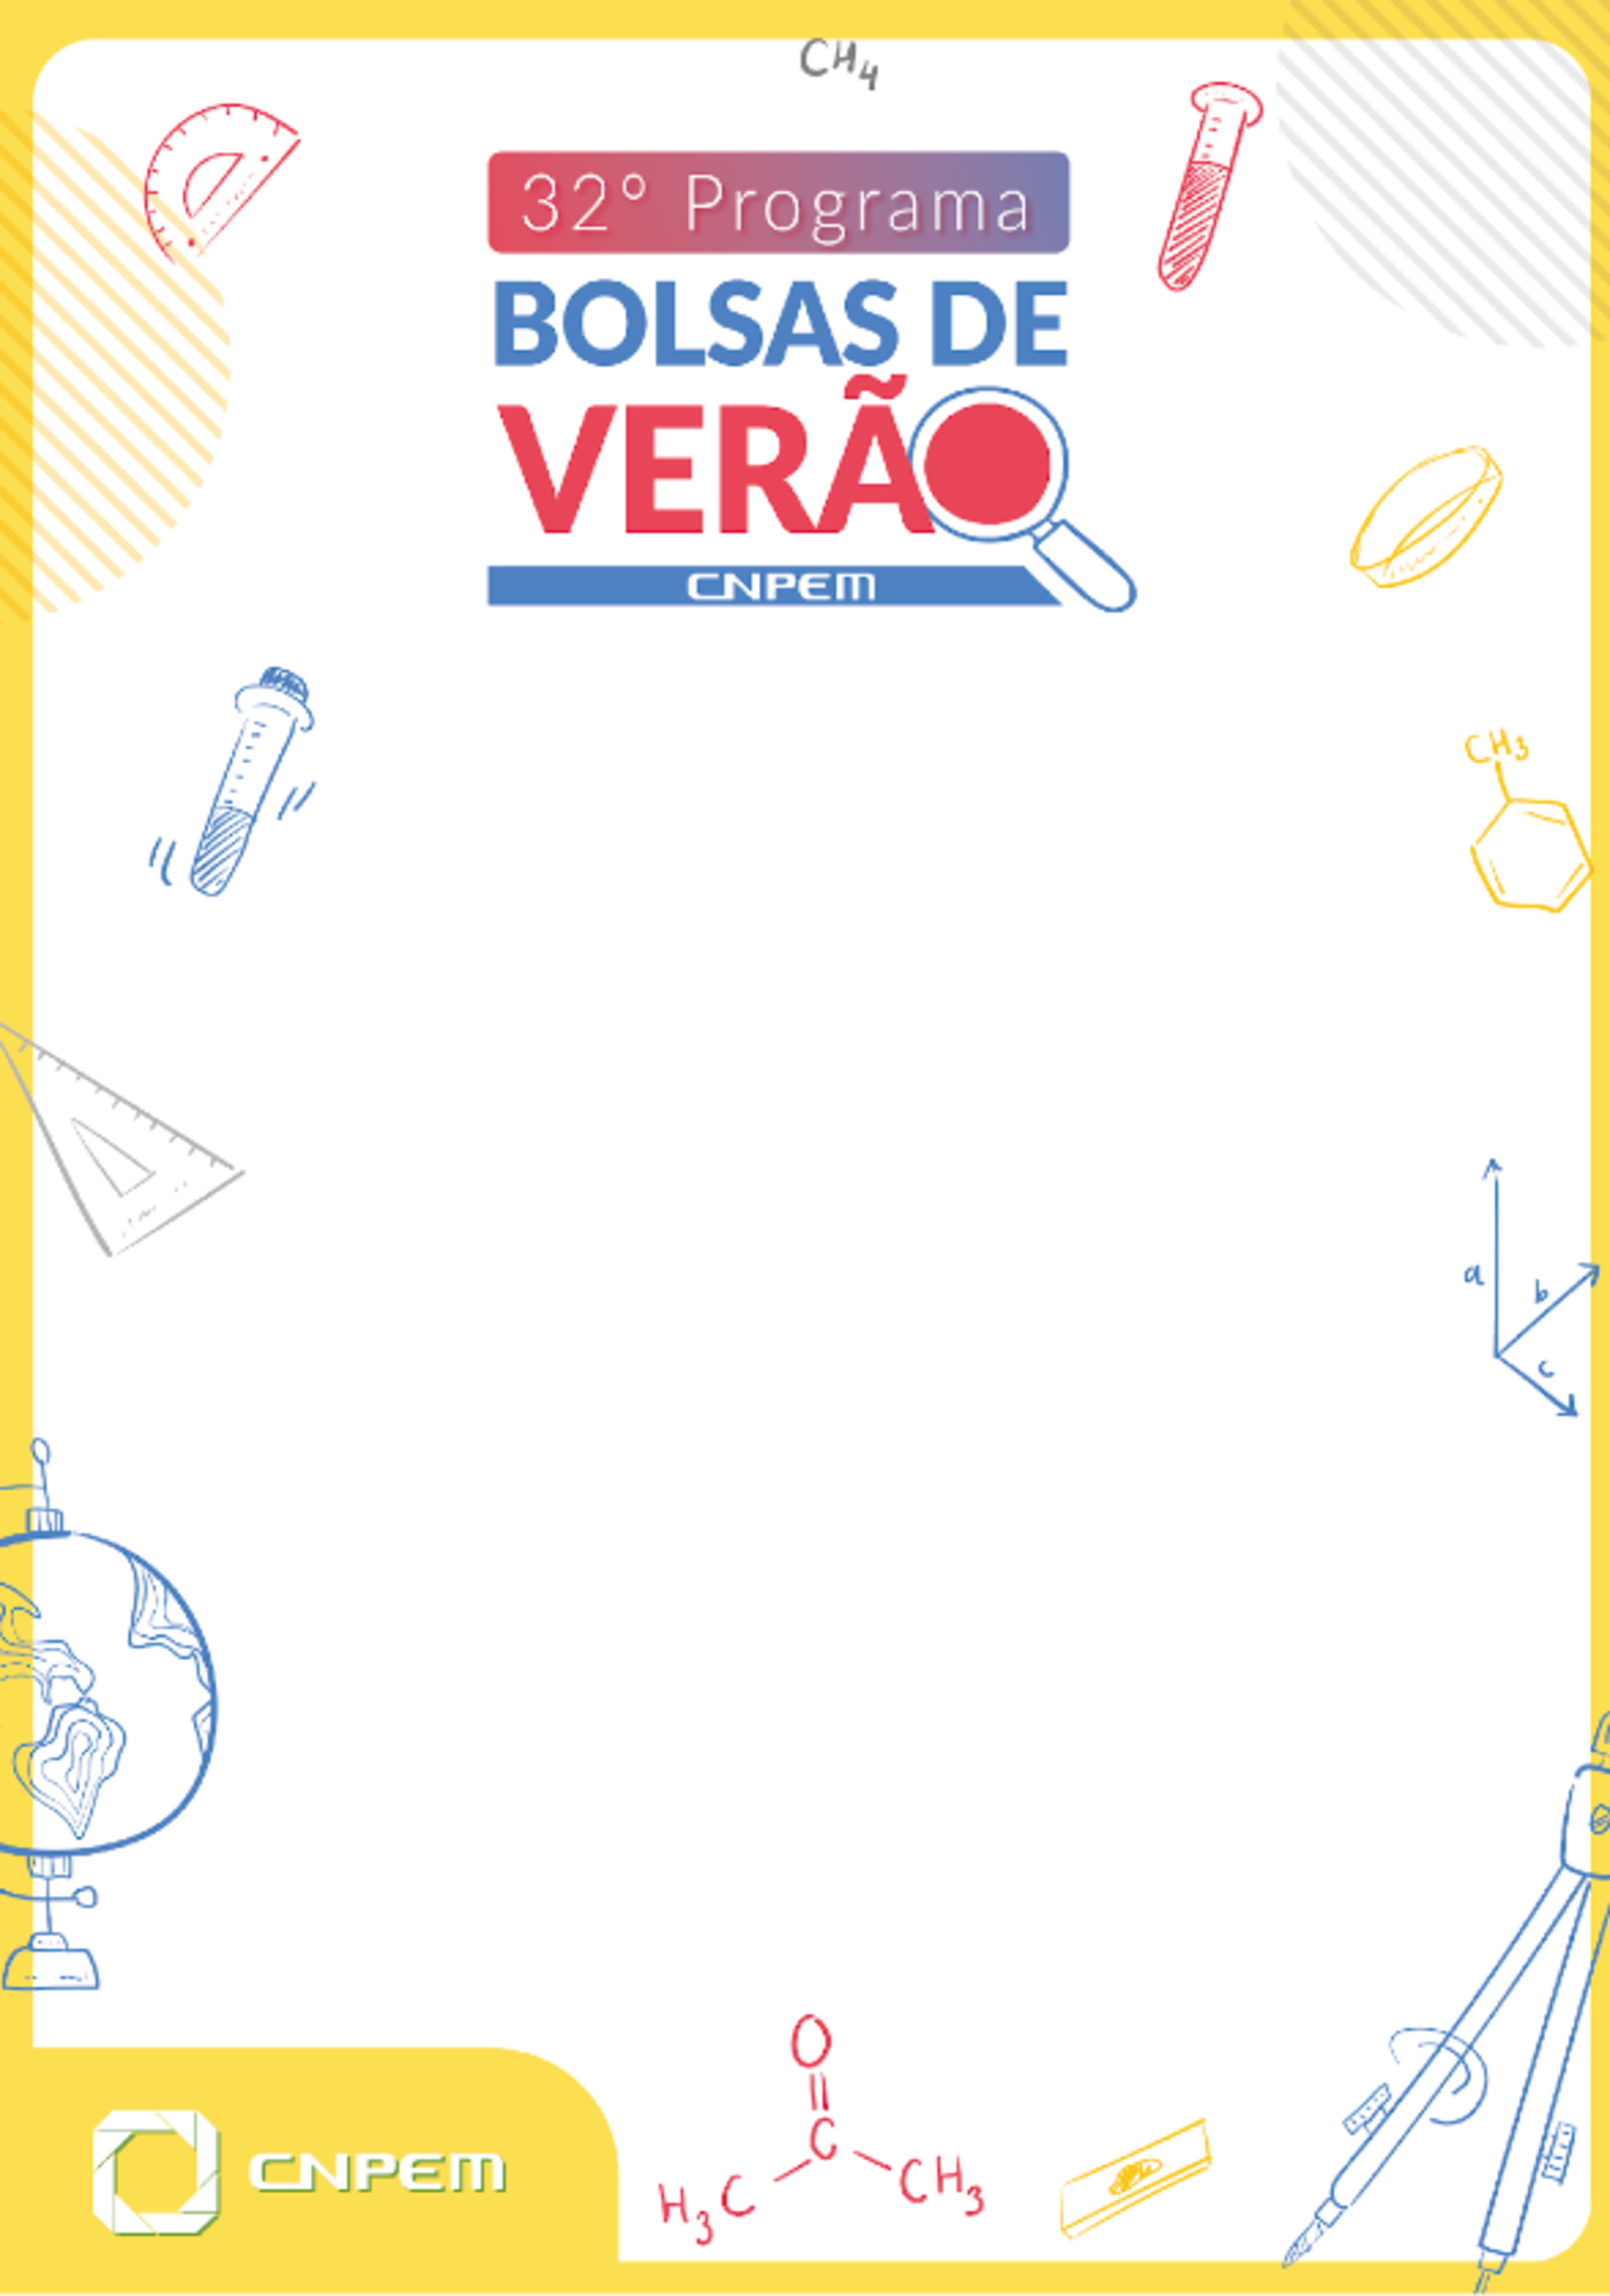
\includegraphics[width=\paperwidth,height=\paperheight]{Pictures/Cover.png}} % Background image (page 1)
}
\newgeometry{margin=0cm}
\begin{titlepage}
\centering
\vspace*{0.35\textheight}
{\textcolor{red}{\Huge \textbf{Accessing the structure of \\ metal/zeolite catalyst by \\combining 3D imaging \\ and high resolution microscopy\\ techniques}}} % Title in red and large
\vspace{2cm}
\Large

\textbf{\textit{Bolsista:}} \textit{Your name}\\[0.5em] % Your name
 \textit{\textbf{Career:}} \textit{Your career} \\[0.5em] %Your Carrer
 \textit{\textbf{University:}} \textit{Your university} \\[0.5em] %Your university
 \textit{\textbf{Advisor}} \textit{Your advisor} %Your counselor
\end{titlepage}
\restoregeometry

%                      %%--- Different background for second page ---%%%
\clearpage
\backgroundsetup{
 scale=1,
 angle=0,
 opacity=1,
 contents={
\includegraphics[width=\paperwidth,height=\paperheight]{Pictures/Intermediate.png}}
}
                       %%--- Different background for last page ---%%%
\vspace{10cm}
\tableofcontents

%%%------------------------------------- Index ------------------------------%%%
\newpage
\section*{Abstract}
\addcontentsline{toc}{section}{Abstract} 
% Here goes the content of the "Abstract" section of the PDF

\section*{Contextualization}
\addcontentsline{toc}{section}{Contextualization}
% Here goes the content of the "Contextualization" section of the PDF


\section{Introduction}
% Here goes the content of the "Introduction" section of the PDF
% This is a text that was generated randomly with a Latex package, with the purpose of expressing how bibliographic citation works. You can remove it and add your introduction with its proper citations. 
\lipsum[2] \textcite{example2}
\lipsum[4]\textcite{example1}


\section{Objectives}
% Here goes the content of the "Objectives" section of the PDF

% Write your general objective here
\subsection{General Objective}

% Write your specific objectives here
\subsection{Specific Objectives}


\section{Methods}
% Here goes the content of the "Methods" section of the PDF

\section{Results and discussion}
% Here goes the content of the "Results and discussion" section of the PDF

\section{Conclusions}
% Here goes the content of the "Conclusions" section of the PDF



\addcontentsline{toc}{section}{References} 
\printbibliography

%%%---%%%---%%%---%%%-----------  End index  -------------------%%%---%%%---%%%---%%%
\newpage
\backgroundsetup{
scale=1, % Image scale
angle=0, % Image angle
opacity=1, % Image opacity
contents={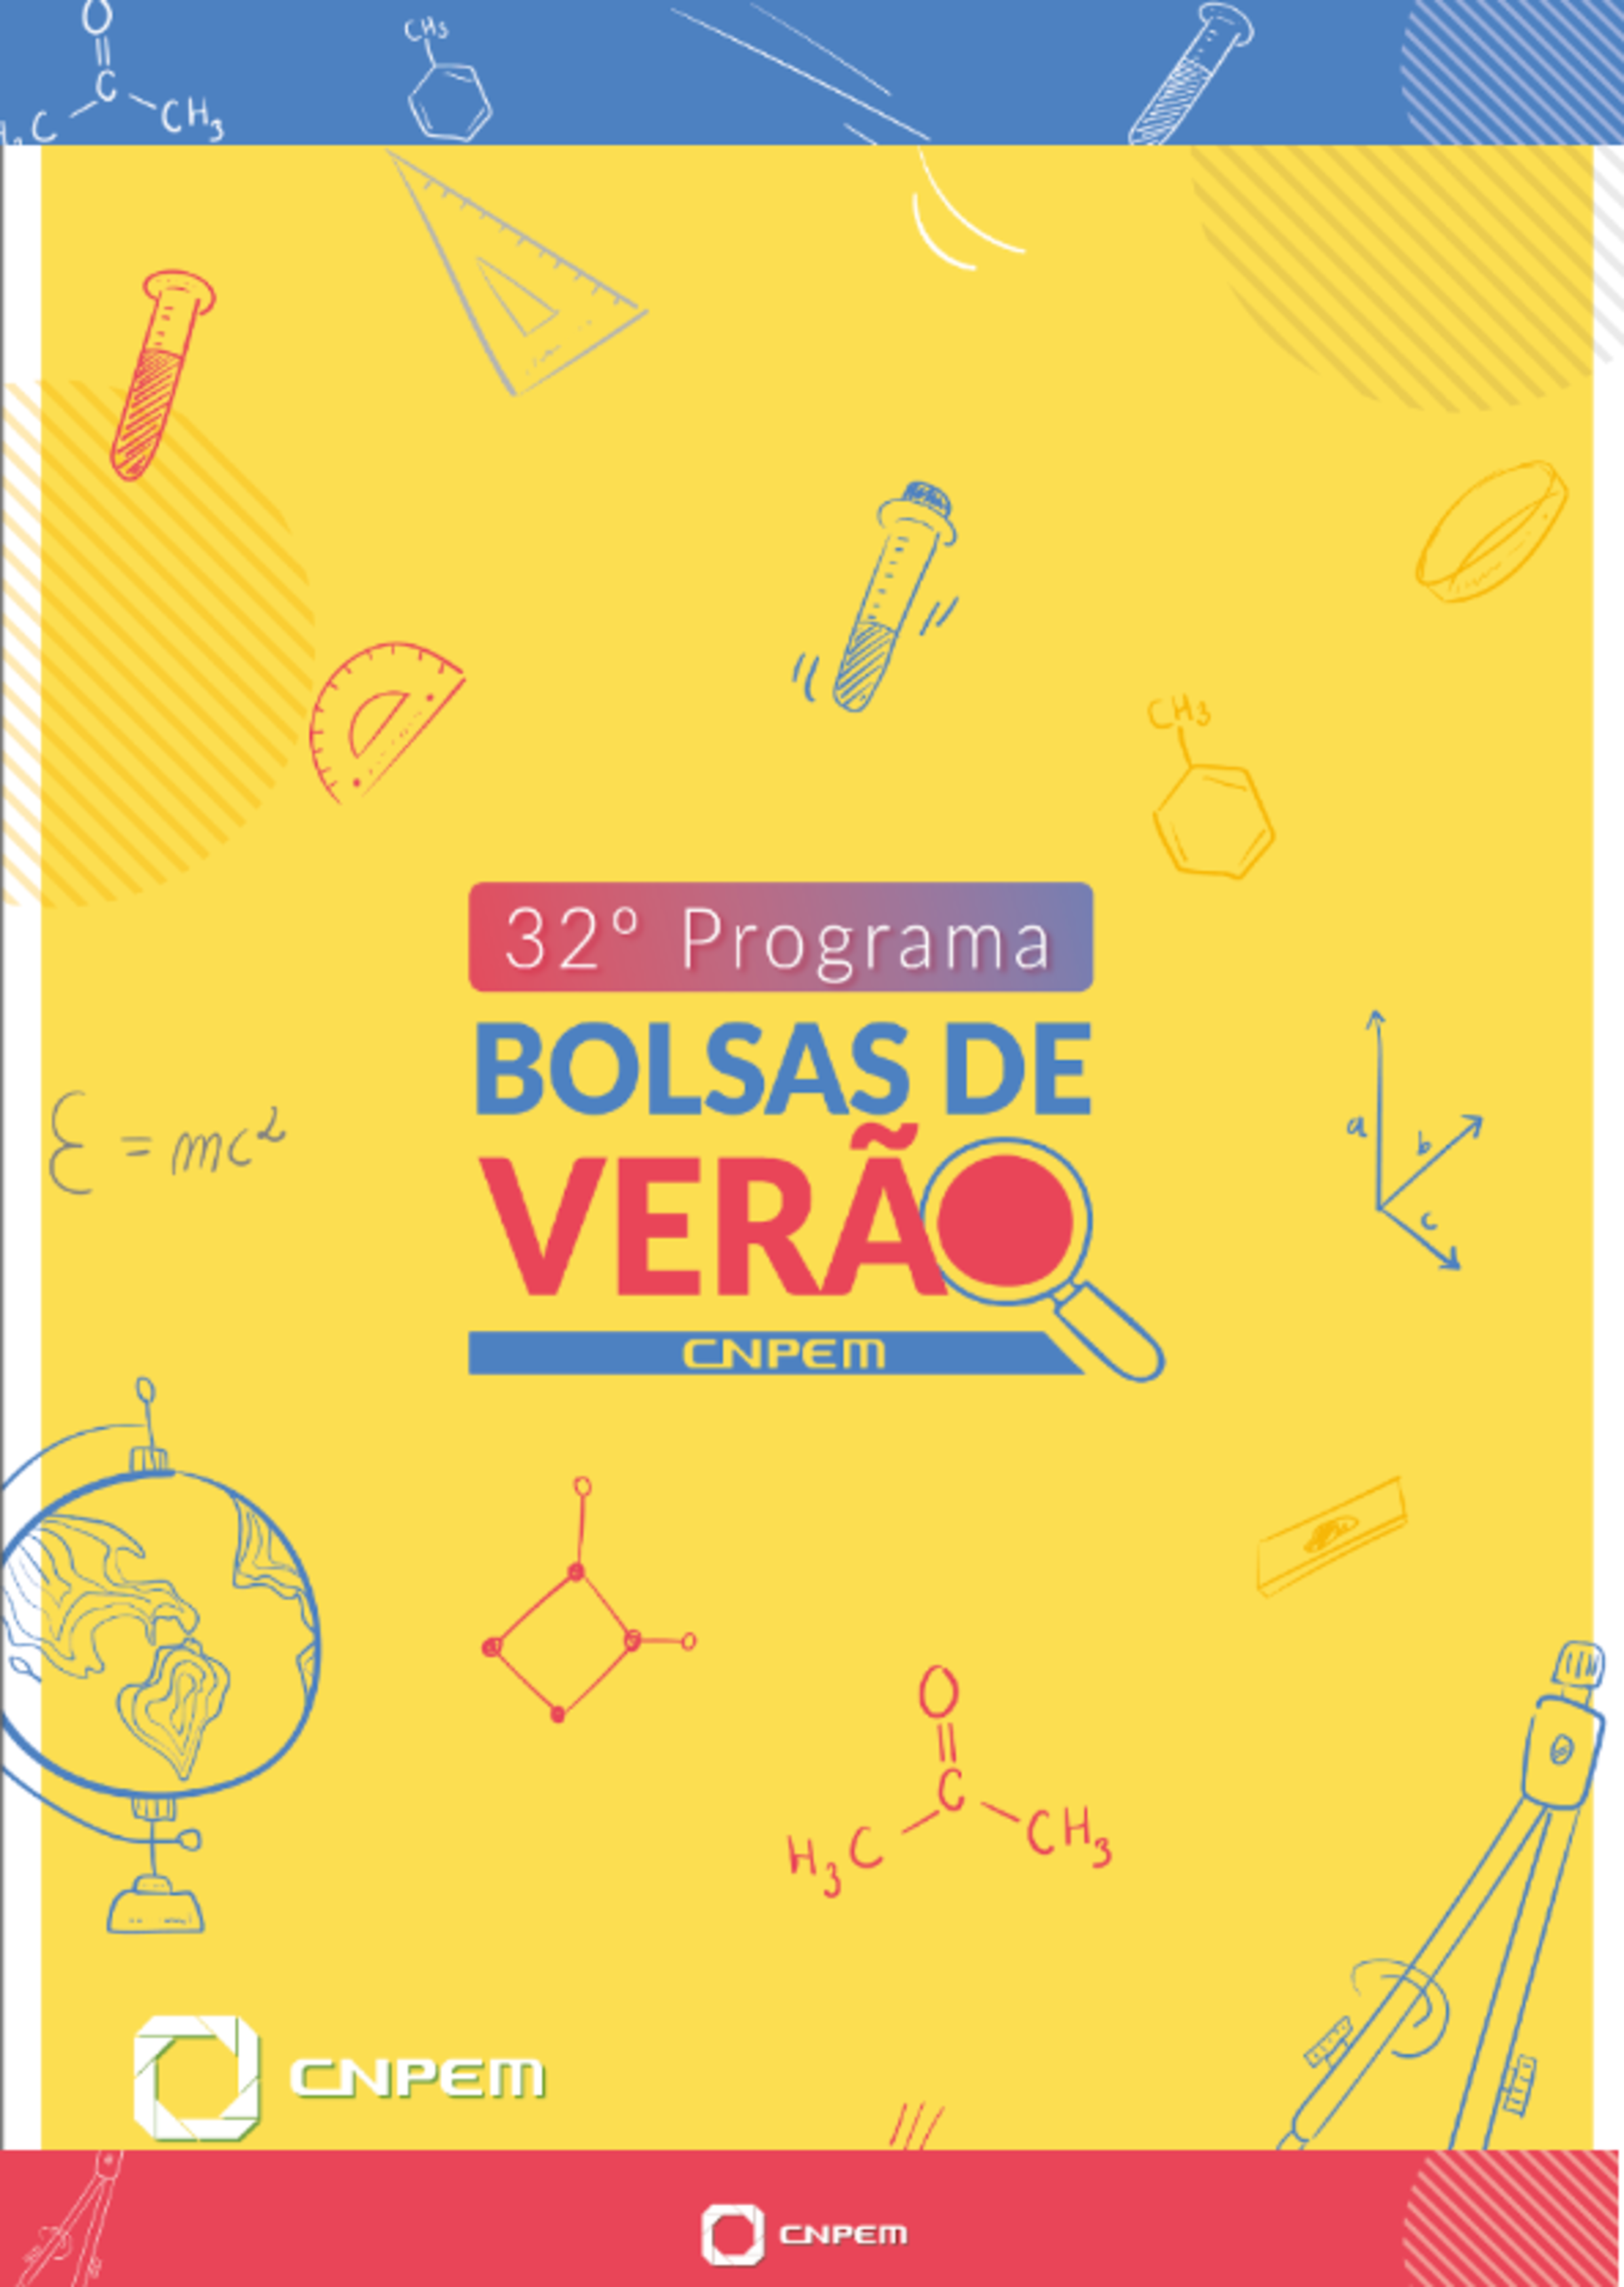
\includegraphics[width=\paperwidth,height=\paperheight]{Pictures/Cover_e.png}} % Background image for the last page
}
\begin{center}
% If you need additional text on the last page, you can add it here
\vspace*{\fill}
{\Huge \textbf{}}
\vspace*{\fill}
\end{center}

\end{document}